% Template from the DPHPC course website

% IEEE standard conference template; to be used with:
%   spconf.sty  - LaTeX style file, and
%   IEEEbib.bst - IEEE bibliography style file.
% --------------------------------------------------------------------------

\documentclass[letterpaper]{article}
\usepackage{spconf,amsmath,amssymb,graphicx}
\usepackage[english]{babel}
\usepackage[utf8]{inputenc}
\usepackage{verbatim}		
\usepackage{epstopdf}
\usepackage[font=footnotesize]{caption}
\usepackage[dvipsnames]{xcolor}
\usepackage{hyperref}
\usepackage{listings}	
\usepackage{multicol}
\usepackage{ifthen}
\usepackage{tikz}
\usetikzlibrary{arrows,decorations.pathmorphing,backgrounds,fit,positioning,shapes.symbols,chains,calc,shapes}

% Example definitions.
% --------------------
% Nice typeset for C++
\newcommand{\Cpp}{C\nolinebreak[4]\hspace{-.05em}\raisebox{.2ex}{\small \bf ++}}
%\newcommand{\Cpp}{C\nolinebreak\hspace{-.05em}\raisebox{.4ex}{\tiny\bf +}\nolinebreak\hspace{-.10em}\raisebox{.4ex}{\tiny\bf +}}
%\newcommand{\Cpp}{\texttt{C\nolinebreak+\nolinebreak+}}


% bold paragraph titles
\newcommand{\mypar}[1]{{\bf #1.}}

% For example:
% ------------
%\address{School\\
%		 Department\\
%		 Address}
%
% Two addresses (uncomment and modify for two-address case).
% ----------------------------------------------------------
%\twoauthors
%  {A. Author-one, B. Author-two\sthanks{Thanks to XYZ agency for funding.}}
%		 {School A-B\\
%		 Department A-B\\
%		 Address A-B}
%  {C. Author-three, D. Author-four\sthanks{The fourth author performed the work
%		 while at ...}}
%		 {School C-D\\
%		 Department C-D\\
%		 Address C-D}
%


\ifthenelse{\boolean{true}}% TODO: change to false to hide invisible notes
{ \newenvironment{invisible}{\par\bigskip\color{gray}}{\par\bigskip} }%
{ \newenvironment{invisible}{\expandafter\comment}{\expandafter\endcomment} }

\title{Topological Sorting: A Parallel Implementation}

\name{J. Baum, K. Wallimann, M. Untergassmair}%
\address{ETH Zürich, HS 2015 \\
	Design of Parallel and High Performance Computing \\
	Zürich, Switzerland}

%%%%%%%%%%%%%%%%%%%%%%%%%%%%%%%%%%%%%%%%%%%%%%%%%%%%%%%%%%%%%%%%%%%%%%%%%%%%%%%%


	
	
	
\begin{document}

\maketitle

\begin{abstract}
 We can already start putting some theory parts in the report right now, so it's easier later to get everything together\ldots \\
Formatting comes later.
\end{abstract}


\begin{invisible}
	This will not be in final report \\
	we can put derivations and remarks here
\end{invisible}

\section{Introduction}\label{sec:intro}

\mypar{Motivation}
\begin{invisible}
  \begin{itemize}
  \item Software Dependencies
  \item Maybe, to flesh out: Admittedly a bit academic, but interesting problem nevertheless, because memory bound => This is the future of HPC
  \end{itemize}
\end{invisible}


\mypar{Related work} 
\begin{invisible}
  \begin{itemize}
  \item MC Er Paper \cite{er1983parallel}: Unclear how to retrieve a sorted list from values without sorting and threads might chase other threads. No words about load balancing => Not practicable
  \item Ma Paper \cite{ma1997efficient}: Theoretical analysis in PRAM model, not practicable.
  \item Both cases: No code
  \item Our contribution: (1) Modified algorithm based on MC Er. 1. Sorted list is directly extracted. 2. only one thread continues when multiple threads meet. 3. Ensure load balancing
                          (2) Actual implementation for shared memory architecture
  \end{itemize}
\end{invisible}


\section{Background: Whatever the Background is}\label{sec:background}
%TODO: Johannes

 In this section, we define the topological sort problem and contrast it to BFS and DFS.
 Furthermore, we introduce the basics of the parallel algorithms we use (and a cost analysis?).
 \\
 

\mypar{Topological sorting}
A directed graph can be seen as a binary relation. If the graph is also acyclic it describes a partial order and it is called a directed acyclic graph (DAG). A topological sorting is a total order on a DAG. Let $G = (V,E)$ be a DAG where $V$ is the set of vertices and $E$ is the set of edges. Formally a topological sorting is a function $ord: V \longrightarrow \{1,...,n\}$ where $n = |V|$ such that $\forall (v,w) \in E: ord(v) \leq ord(w)$.
Figure \ref{fig:ts-example} shows a DAG with a corresponding topological sorting: A,I,F,B,E,D,H,G,C. Even though every DAG has at least one topological sorting, mostly there are many different topological sortings for the same graph.

\begin{figure}[!hbp]
 \centering
  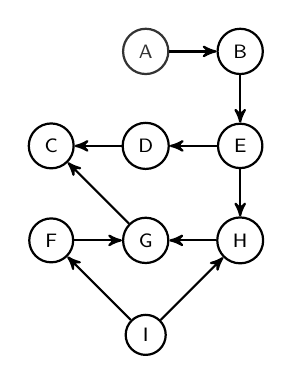
\begin{tikzpicture}[->,>=stealth',auto,node distance=1cm,
                    thick,main
                    node/.style={circle,draw,font=\sffamily\scriptsize},text node/.style={draw=none,font=\sffamily\tiny}]

  \node[main node] (1) [draw=black!80,text=black!80] {A};
  \node[main node] (3) [right of=1, node distance=1.2cm]{B};
  \node[main node] (7) [below of=3, node distance=1.2cm] {E};
  \node[main node] (4) [left of=7, node distance=1.2cm] {D};
  \node[main node] (5) [below of=7, node distance=1.2cm] {H};
  \node[main node] (6) [left of=4, node distance=1.2cm] {C};
  \node[main node] (8) [left of=5, node distance=1.2cm] {G};
  \node[main node] (9) [below of=8, node distance=1.2cm] {I};
  \node[main node] (2) [left of=8, node distance=1.2cm] {F};
  


  


  \path[every node/.style={font=\sffamily\small}]
    (1) edge (3)
    (3) edge (7)
    (7) edge (4)
    (4) edge (6)
    (7) edge (5)
    (5) edge (8)
    (8) edge (6)
    (9) edge (5)
    (9) edge (2)
    (2) edge (8)
    ;
\end{tikzpicture}

\caption{Example DAG where A,I,F,B,E,D,H,G,C is one possible topological sorting}
\label{fig:ts-example}
\end{figure}

Topological sortings are often beeing used to schedule tasks based on their dependencies. Every vertice represents a task and the edges represent the relation between the tasks.

Although the results of the breadth-first-search (BFS) algorithm seem to be similar to topological sortings, they are not equivalent. BFS and topolocical sorting algorithms both yield a sequence of nodes, containing each node exactly once. The important difference between the results of BFS and a topological sorting is, that a topological sorting is a total order with respect to the partial order represented by the input graph. But BFS can also return sequences which are not total orders. A simple example is shown in figure \ref{fig:diff-bfs}. The visiting sequence A,C,B is valid in BFS but is not a topological sorting. The only valid topological sorting for the example graph is A,B,C.


\begin{figure}[!hbp]
\centering
 
  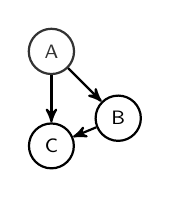
\begin{tikzpicture}[->,>=stealth',auto,node distance=1cm,
                    thick,main
                    node/.style={circle,draw,font=\sffamily\scriptsize},text node/.style={draw=none,font=\sffamily\tiny}]

  \node[main node] (1) [draw=black!80,text=black!80] {A};
  \node[main node] (2) [below right of=1, node distance=1.2cm]{B};
  \node[main node] (3) [below of=1, node distance=1.2cm] {C};
  

  \path[every node/.style={font=\sffamily\small}]
    (1) edge (2)
    (2) edge (3)
    (1) edge (3)
    ;
\end{tikzpicture}

\caption{A,C,B is a valid sequence in breadth-first-search (BFS) and depth-first-search (DFS) but not a topological sorting}
\label{fig:diff-bfs}
\end{figure}

A sequential algorithm yielding a topological sorting has been suggested by Kahn \cite{kahn1962topological}. Another algorithm has been published by Tarjan  \cite{tarjan1976edge} and is based on depth-first-search (DFS). Both algorithms have an asymptotic complexity of $\mathcal{O}(|V|+|E|)$. It is to mention that DFS alone does not necessarily return a topological sorting. This can be shown with the same argument as for BFS using figure \ref{fig:diff-bfs}.

 \mypar{Parallel algorithm} 
 1983 M. C. Er \cite{mcer1983} came up with a parallel approach to retrieve a topological sorting. The algorithm works in 5 steps:
 \begin{enumerate}
 	\item Build the graph from the given partial order (optional if the problem is already stated as a graph).
 	\item Add a special node value to every node and initialize it to zero
 	\item Visit all source nodes (nodes with an indegree of zero) and set their node values to one.
 	\item Start from all source nodes in parallel and proceed with all successor nodes as follows: Let $N_p$ be the node value of the current source node and $N_s$ the node value of the currently observed successor node. Then the algorithm checks if $N_s \leq N_p$ and sets the value of the successor to $N_p + 1$, if so. This step is iterated until there are no further successor nodes. If during this step a value higher than the total amount of nodes is beeing assigned to a node, this means that the input graph is not acyclic and the algorithms stops.
 	\item List all the nodes in ascending order of node values.
 \end{enumerate}

The correctness of the algorithm relies on another condition. To avoid the situation that two processes or threads try to update a node value at the same time with different values, M. C. Er proposes a synchronization after every step. This results in the fact that if two processes or threads try to update the same node's value, they want to write the same value. This is because they must be at the same iteration step due to the proposed barrier synchronization. This comes at the price of a lower performance. Also with this approach several processes or threads could follow the same paths in the graph because there is no mechanism preventing a process or thread of following a path which already has been processed by another process or thread.

The asymptotic parallel runtime of the above algorithm is described by M. C. Er as $\mathcal{O}(D_{max})$, where $D_{max}$ is defined as the maximum distance between a source node and a sink node. This runtime is hard to achieve in practice if one implements step 5 of the algorithm via sorting the nodes with respect to their values. It is not mentioned by M. C. Er how to create the result list of step 5.


\mypar{Improvements} 
The approach proposed in this report does not use node values. Instead the node is directly put into the solution list. This avoids having to sort the nodes by their value at the end. Also the barriers are not necessary anymore. However, it must be made sure that no node is written more than once to the result list and race conditions while writing to the solution list must be avoided. This approach addresses the problem of several processes following the same path with introducing a parent counter. This counter is a special value of each node, stating how many parent nodes it has. At the beginning this value is set to the actual amount of parents. During the algorithm each process arriving at a node will decrease the counter by one. It will only follow the node if the parent counter is zero. Thus only the last arriving process will follow the path. It has to be taken care of the possible race condition while updating the parent counter.



 
 
 
 \begin{invisible}
 % Serial TS
 \mypar{Topological sorting}
 \begin{itemize}
  \item What is topological sort, difference to BFS
  \item Input: A set of dependencies (aka partial orders) of the form A $\rightarrow$ B ``A must come before B''
  \item Output: A sequence (aka total order) containing all nodes exactly once. All partial orders must be kept.
  \item Solution not unique
  \item Minimal Example: A->B, A->C, B->C. Valid BFS traversal order: A, C, B. Invalid for TS.
  \item TS can (serially) be solved with Kahn's algorithm \cite{kahn1962topological} or DFS and Backpropagation (Tarjan \cite{tarjan1976edge}). % See Wikipedia
        Note that TS is not equivalent to DFS, e.g. for A->B, B->C, A->D, D->E, DFS and Backpropagation yields A, B, C, D, E, but another valid TS is A, B, D, C, E
  \item Asymptotic runtime: O(|V| + |E|)
As an aside, don't talk about "the complexity of the algorithm.'' It's incorrect,
problems have a complexity, not algorithms.  
 \end{itemize}

 % Multithreaded TS
 \mypar{Parallel algorithm}
 \begin{itemize}
  \item Short overview over algorithm of MC Er
  \item Parallelization over child nodes
  \item His idea with barrier in each step such that even if the index is written by multiple threads, they write the same number => Avoid race condition at writing the index
  \item Our idea: Instead of writing an index, directly write to solution list. As a consequence, we have to make sure that node is written to solution only once. And of course there is a race condition on writing to solution list.
  \item Our idea: First, count (in parallel) how many parents each node has. Each time a node is visited, decrement counter and only write to solution if counter is zero. Of course, there is a race condition on the parent counter.
  \item 3 synchronization points (that is, bottlenecks): 1. Barrier after each level, 2. Lock solution list for appending new nodes, 3. Lock parent counter for decrementing it and checking if it is zero.
  \item Cost
 \end{itemize}

 
\end{invisible}

%TODO: Change title
\section{Your Proposed Method}\label{sec:yourmethod}
%TODO: Kevin
In this section, we present different implementations of the parallel algorithm outlined above.
Especially, we show how to efficiently implement the three synchronization points and how to ensure load balancing.

\begin{invisible}
Somewhere, we need to mention that we are working with an adjacency list.
 \mypar{Efficient update of solution list} %locallist, worksteal, bitset
 \begin{itemize}
  \item Thread-local solution lists over one level.
  \item Append whole list to global list instead of appending each node individually. Order across one level doesn't matter.
  \item Same level ensured thanks to barrier. Global solution sequence must be a list, can't be a vector.
 \end{itemize}

 %TODO: Better title
 \mypar{Efficiently decrementing and checking the parent counter} %locallist, worksteal, bitset, dynamic_nobarrier
 Insert code of CAS-version of requestValueUpdate
 
 \mypar{Barrier-free implementation} %dynamic_nobarrier
 \begin{itemize}
  \item Don't use barrier at all. MC Er only used it to avoid race conditions at writing indices.
  \item We lock the solution list, so there should be no race condition. But: Cannot use thread-local solution lists anymore.
 \end{itemize}

 \mypar{Load balancing}
 \begin{itemize}
  \item Parallelization over front $\Rightarrow$ Load balancing also over front. Two distinct representations of front: Using thread-local lists and using a global bitset.
  \item Thread-local lists: Following an idea described in \cite{bulucc2011parallel} %@matthias: Siehe 4.2 Shared memory computation Stichwort thread-local stacks. Müssen das nicht zitieren, weil wir die Idee ja unabhängig gefunden haben.
  For each level, distribute children evenly among threads. Each thread then holds a list of children that it processes.
  At the same time, it creates a list of new children which are collected and redistributed at the next level.
  \item Work stealing: Based on thread-local lists, but better redistribution of nodes?
  \item Bitset: Idea used in e.g. \cite{agarwal2010scalable} or \cite{beamer2013direction}. Loop over bitset, do nothing if bit is zero. Load balancing with dynamic scheduler of OpenMP.
  New children are written into a separate bitset. At the end of a level, bitsets are swapped.
 \end{itemize}

\end{invisible}

\section{Experimental Results}\label{sec:exp}
%TODO: Matthias
In this section, we present our experimental setup and the impact of the different optimizations and implementations described in the previous section.

\begin{invisible}
 \mypar{Experimental setup}
 \Cpp  OpenMP
 (processor, frequency, maybe OS, maybe cache sizes)
 compiler, version, and flags used.
 %TODO: Should we play with optimization flags?

 \mypar{Benchmarks}
 For each item, mention graph type, number of nodes, node degree, optimizations from above
 \begin{itemize}
  \item Influence of barrier. Introduce multichain graph, Strong Scaling dynamic nobarrier opt2 MULTICHAIN100 vs bitset global opt1 MULTICHAIN100 Why Multichain100: Should be dominated by barrier%bitset_global is bitset without local solutions, because dynamic_nobarrier has no local solutions
  \item Influence of local solution. Strong Scaling bitset MULTICHAIN10000 vs bitset global MULTICHAIN10000 Why Multichain10000: Should be dominated by pushbacks to solution
  \item Influence of atomic counter check. Strong Scaling RANDOMLIN 100000 opt = true vs opt = false for worksteal and bitset
  \item Strong Scaling software graph \cite{musco2014generative}
  \item Strong Scaling random graph with different degrees
  \item Vertex Scaling plot random graph
 \end{itemize}

\mypar{Results}

Questions to each plot
\begin{itemize}
 \item What is the performance penalty of the barrier?
 \item How well performs the local solution compared to locking the 
 \item How does the atomic counter check scale compared to the locked version?
 \item How does the best version of our code scale on a real-world example?
 \item How does the best version of our code scale in a slightly artificial scenario?
\end{itemize}
\end{invisible}


\section{Conclusions}

\begin{invisible}
 \begin{itemize}
   \item Best thing would be to have no barriers and still local solution update
   \item Since this is not possible, it is better to accept barriers so as to benefit from local solution
   \item It is worth noting that performance highly depends on the structure of the graph.
 \end{itemize}
\end{invisible}

% References should be produced using the bibtex program from suitable
% BiBTeX files (here: bibl_conf). The IEEEbib.bst bibliography
% style file from IEEE produces unsorted bibliography list.
% -------------------------------------------------------------------------
\bibliographystyle{IEEEbib}
\bibliography{bibliography}



\end{document}
